\documentclass[10pt]{beamer}
\usetheme{metropolis}

% ── Packages ──
\usepackage{amsmath,amssymb,amsthm}
\usepackage{tikz}
\usetikzlibrary{positioning,arrows.meta,fit,matrix}
\usepackage{graphicx}
\usepackage{array}
\usepackage{etoolbox}

% ── Theorem environments ──
\theoremstyle{definition}
\newtheorem{defi}{Definition}[section]
\newtheorem{prop}{Proposition}[section]
\newtheorem{thm}{Theorem}[section]
\newtheorem{cor}{Corollary}[section]

% Custom theorem styles with colors
\setbeamercolor{block title}{bg=red!75!black,fg=white}
\setbeamercolor{block body}{bg=yellow!10!white}

% Proposition uses yellow title
\AtBeginEnvironment{prop}{%
  \setbeamercolor{block title}{bg=yellow!75!black,fg=black}%
  \setbeamercolor{block body}{bg=yellow!10!white}%
}
\AtEndEnvironment{prop}{%
  \setbeamercolor{block title}{bg=red!75!black,fg=white}%
}

% ── Emoji definitions ──
\newcommand{\bean}{
\includegraphics[scale=0.07]{Pictures/bean.png}}
\newcommand{\leaf}{
\includegraphics[scale=0.08]{Pictures/leaf.png}}
\newcommand{\lemon}{
\includegraphics[scale=0.08]{Pictures/lemon.png}}
\newcommand{\cow}{
\includegraphics[scale=0.08]{Pictures/cow.png}}
\newcommand{\milk}{
\includegraphics[scale=0.08]{Pictures/milk.png}}
\newcommand{\coffee}{
\includegraphics[scale=0.08]{Pictures/coffee.png}}
\newcommand{\tea}{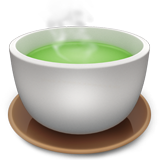
\includegraphics[scale=0.08]{Pictures/tea.png}}
\newcommand{\bento}{
\includegraphics[scale=0.08]{Pictures/bento.png}}
\newcommand{\ramen}{\includegraphics[scale=0.08]{Pictures/ramen.png}}
\newcommand{\cola}{
\includegraphics[scale=0.08]{Pictures/cola.png}}

% ── Highlighting ──
\newcommand{\x}[1]{\alert{\textbf{#1}}}

\title{Lecture 5: Solving Linear Equations and Null Space}
\subtitle{MATH203 Applied Linear Algebra}
\date{}

\begin{document}
\maketitle

% ═══════════════════════════════════════
% §0 MOTIVATION
% ═══════════════════════════════════════
\section{Motivation: Why We Need to Solve Equations}

\begin{frame}{Recall: The Two Languages (Lecture 4)}

Every subspace has \x{two complementary descriptions}:

\vspace{1em}

\begin{center}
\begin{tabular}{|c|c|c|}
\hline
\textbf{Language} & \textbf{How it works} & \textbf{Example} \\
\hline
\x{Descriptive} & List \textbf{equations} & $\{\mathbf{x} : A\mathbf{x} = \mathbf{0}\}$ \\
 & (constraints) & \\
\hline
\x{Constructive} & Provide \textbf{recipe} & $\text{span}\{\mathbf{v}_1, \mathbf{v}_2, \ldots\}$ \\
 & (generate members) & \\
\hline
\end{tabular}
\end{center}

\vspace{1em}

\x{Today's question}: What is each language \textbf{good at}? What is each language \textbf{bad at}?

\end{frame}

\begin{frame}{Each Language Has Strengths and Weaknesses}

\begin{center}
\begin{tabular}{|c|c|c|}
\hline
& \x{Descriptive} & \x{Constructive} \\
& $\{\mathbf{x} : A\mathbf{x} = \mathbf{0}\}$ & $\text{span}\{\mathbf{v}_1, \ldots\}$ \\
\hline
\textbf{Good at} & Verification & Generation \\
 & (check membership) & (produce members) \\
\hline
\textbf{Bad at} & Generation & Verification \\
 & (find examples) & (check membership) \\
\hline
\end{tabular}
\end{center}

\vspace{1em}

\x{Key insight}: \textbf{Solving equations helps both languages do what they're bad at!}

\vspace{1em}

Let's see two concrete examples$\ldots$

\end{frame}

\begin{frame}{Example Setup: Shinchan's Coffee Shop Menu}

Shinchan has three drinks on his menu:

\vspace{0.5em}

\begin{center}
\begin{tabular}{c|ccc}
& \milk & \coffee & \tea \\
\hline
\leaf & 0 & 0 & 2 \\
\lemon & 0 & 0 & 1 \\
\bean & 0 & 2 & 4 \\
\cow & 1 & 0 & 1 \\
\end{tabular}
\end{center}

\vspace{0.5em}

Matrix form:
$$A = \begin{pmatrix}
0 & 0 & 2 \\
0 & 0 & 1 \\
0 & 2 & 4 \\
1 & 0 & 1
\end{pmatrix}$$

We'll use this matrix $A$ to illustrate \x{both cases}.

\end{frame}

\begin{frame}{Case 1: Column Space (Naturally Constructive)}

The column space is \x{naturally constructive}:

$$\text{Col}(A) = \text{span}\left\{\begin{pmatrix} 0\\0\\0\\1 \end{pmatrix}, \begin{pmatrix} 0\\0\\2\\0 \end{pmatrix}, \begin{pmatrix} 2\\1\\4\\1 \end{pmatrix}\right\}$$

\vspace{1em}

\x{Generation} (easy): Want a vector in $\text{Col}(A)$? Pick coefficients!

$$2\begin{pmatrix} 0\\0\\0\\1 \end{pmatrix} + 3\begin{pmatrix} 0\\0\\2\\0 \end{pmatrix} = \begin{pmatrix} 0\\0\\6\\2 \end{pmatrix} \in \text{Col}(A)$$

\end{frame}

\begin{frame}{Case 1: Column Space Needs Solving for Verification}

\x{Verification} (hard): Is $\mathbf{b} = \begin{pmatrix} 4\\2\\10\\3 \end{pmatrix}$ in $\text{Col}(A)$?

\vspace{1em}

Can't tell by looking! Need to \x{solve}: $A\mathbf{x} = \mathbf{b}$

\vspace{1em}

\begin{itemize}
\item If solution exists $\Rightarrow$ $\mathbf{b} \in \text{Col}(A)$ \checkmark
\item If no solution $\Rightarrow$ $\mathbf{b} \notin \text{Col}(A)$ $\times$
\end{itemize}

\vspace{1em}

\x{Solving equations gives constructive description the power to verify!}

\end{frame}

\begin{frame}{Case 2: Null Space (Naturally Descriptive)}

The null space is \x{naturally descriptive}:

$$\text{Null}(A) = \{\mathbf{x} \in \mathbb{R}^3 : A\mathbf{x} = \mathbf{0}\}$$

\vspace{1em}

\x{Verification} (easy): Is $\mathbf{v} = \begin{pmatrix} 0\\1\\-2 \end{pmatrix}$ in $\text{Null}(A)$?

\vspace{0.5em}

Just compute:
$$A\begin{pmatrix} 0\\1\\-2 \end{pmatrix} = \begin{pmatrix} -4\\-2\\-6\\0 \end{pmatrix} \neq \mathbf{0}$$

Not in null space! (Easy to check!)

\end{frame}

\begin{frame}{Case 2: Null Space Needs Solving for Generation}

\x{Generation} (hard): The columns (\milk, \coffee, \tea) have redundancy.

\vspace{0.5em}

Can you find it by staring?

\begin{center}
\begin{tabular}{c|ccc}
& \milk & \coffee & \tea \\
\hline
\leaf & 0 & 0 & 2 \\
\lemon & 0 & 0 & 1 \\
\bean & 0 & 2 & 4 \\
\cow & 1 & 0 & 1 \\
\end{tabular}
\end{center}

\vspace{0.5em}

Hard to see! Need to \x{solve} $A\mathbf{x} = \mathbf{0}$ to get:

$$\text{Null}(A) = \text{span}\left\{\begin{pmatrix} 0\\2\\-1 \end{pmatrix}\right\}$$

\end{frame}

\begin{frame}{What Does This Null Space Vector Tell Us?}

The vector $\begin{pmatrix} 0\\2\\-1 \end{pmatrix}$ records the dependence relation:

$$0 \cdot \text{\milk} + 2 \cdot \text{\coffee} - 1 \cdot \text{\tea} = \mathbf{0}$$

\vspace{0.5em}

Rearranging:
$$2 \times \text{\coffee} = 1 \times \text{\tea}$$

\vspace{1em}

\x{Aha!} The \tea recipe uses exactly \textbf{twice the ingredients} of \coffee recipe. That's the redundancy!

\vspace{1em}

Now generation is easy: $t\begin{pmatrix} 0\\2\\-1 \end{pmatrix}$ for any $t \in \mathbb{R}$ (all scalar multiples record the same relation).

\vspace{0.5em}

\x{Solving equations gives descriptive description the power to generate!}

\end{frame}

\begin{frame}{Summary: The Power of Solving Equations}

\begin{center}
\begin{tabular}{|c|c|c|c|}
\hline
\textbf{Subspace} & \textbf{Natural form} & \textbf{Weakness} & \textbf{Solving provides} \\
\hline
$\text{Col}(A)$ & Constructive & Verification & Solve $A\mathbf{x}=\mathbf{b}$ \\
 & (span) &  & to verify $\mathbf{b} \in \text{Col}(A)$ \\
\hline
$\text{Null}(A)$ & Descriptive & Generation & Solve $A\mathbf{x}=\mathbf{0}$ \\
 & (equations) &  & to get basis \\
\hline
\end{tabular}
\end{center}

\vspace{1em}

\x{Today's focus}: Develop a \textbf{cross-filling method} to solve $A\mathbf{x} = \mathbf{b}$, which simultaneously:

\begin{itemize}
\item Gives constructive description of $\text{Null}(A)$ (find basis)
\item Checks existence: Does $\mathbf{b} \in \text{Col}(A)$?
\item Determines uniqueness: Is $\text{Null}(A) = \{\mathbf{0}\}$?
\item Finds all solutions when they exist
\end{itemize}

\end{frame}

% ═══════════════════════════════════════
% §1 NULL SPACE
% ═══════════════════════════════════════
\section{Null Space: Starting with the Descriptive Definition}

\begin{frame}{Definition: Null Space}

\begin{defi}[Null Space (Kernel)]
For a matrix $A \in \mathbb{R}^{m \times n}$, the \x{null space} is:

$$\text{Null}(A) = \{\mathbf{x} \in \mathbb{R}^n : A\mathbf{x} = \mathbf{0}\}$$

\textbf{Geometric meaning}: $\text{Null}(A)$ stores all \x{linear dependence relations} among the columns of $A$.

Also called the \x{kernel}, denoted $\ker(A)$.
\end{defi}

\end{frame}

\begin{frame}{Immediate Example: Redundancy in the Menu}

Consider Shinchan's menu matrix:

\begin{center}
\begin{tabular}{c|ccc}
& \milk & \coffee & \tea \\
\hline
\leaf & 0 & 0 & 2 \\
\lemon & 0 & 0 & 1 \\
\bean & 0 & 2 & 4 \\
\cow & 1 & 0 & 1 \\
\end{tabular}
\end{center}

\x{Question}: Are there any redundant recipes? Is one meal just a scaled version of another?

\vspace{0.5em}

Hard to see by staring! But if we find $\mathbf{x} \in \text{Null}(A)$, it will \x{reveal the redundancy}.

\end{frame}

\begin{frame}{What the Null Space Vector Tells Us}

Suppose we found (we'll learn how soon):
$$\mathbf{x} = \begin{pmatrix} 0 \\ 2 \\ -1 \end{pmatrix} \in \text{Null}(A)$$

\vspace{0.5em}

Using the column view of $A\mathbf{x} = \mathbf{0}$:

$$0 \cdot \begin{pmatrix} 0\\0\\0\\1 \end{pmatrix} + 2 \cdot \begin{pmatrix} 0\\0\\2\\0 \end{pmatrix} + (-1) \cdot \begin{pmatrix} 2\\1\\4\\1 \end{pmatrix} = \begin{pmatrix} 0\\0\\0\\0 \end{pmatrix}$$

Rearranging:
$$2 \cdot \begin{pmatrix} 0\\0\\2\\0 \end{pmatrix} = 1 \cdot \begin{pmatrix} 2\\1\\4\\1 \end{pmatrix}$$

\x{In coffee shop terms}: $2 \times \text{\coffee} = 1 \times \text{\tea}$

\end{frame}

\begin{frame}{Key Insight: Null Space as Redundancy Catalog}

\x{Key insight}:

\begin{itemize}
\item $\mathbf{x} = \begin{pmatrix} 0 \\ 2 \\ -1 \end{pmatrix}$ doesn't mean "2 coffees minus 1 tea produces zero ingredients" (nonsense!)
\item It means: \x{\tea = 2×\coffee} (a dependence relation)
\item Think of $\text{Null}(A)$ as the \textbf{"redundancy catalog"}
\end{itemize}

\vspace{1em}

\x{Size of the catalog}:
\begin{itemize}
\item $\text{Null}(A) = \{\mathbf{0}\}$ $\to$ no redundancy $\to$ columns \textbf{linearly independent}
\item $\dim(\text{Null}(A)) = k$ $\to$ there are $k$ independent redundancy relations
\end{itemize}

\end{frame}

\begin{frame}{Null Space is a Subspace}

\begin{prop}
$\text{Null}(A)$ is a subspace of $\mathbb{R}^n$.
\end{prop}

\vspace{0.5em}

\textbf{Quick proof}: Verify the three axioms:

\begin{enumerate}
\item $\mathbf{0} \in \text{Null}(A)$ since $A\mathbf{0} = \mathbf{0}$ \checkmark
\item If $A\mathbf{x}_1 = \mathbf{0}$ and $A\mathbf{x}_2 = \mathbf{0}$, then
$$A(\mathbf{x}_1 + \mathbf{x}_2) = A\mathbf{x}_1 + A\mathbf{x}_2 = \mathbf{0} + \mathbf{0} = \mathbf{0}$$ \checkmark
\item If $A\mathbf{x} = \mathbf{0}$, then
$$A(c\mathbf{x}) = c(A\mathbf{x}) = c\mathbf{0} = \mathbf{0}$$ \checkmark
\end{enumerate}

\end{frame}

\begin{frame}{The Problem: We Need Constructive Description}

As we saw in the motivation, \x{descriptive definitions are good at verification but bad at generation}.

\vspace{1em}

\x{Descriptive definition}: $\text{Null}(A) = \{\mathbf{x} : A\mathbf{x} = \mathbf{0}\}$

\begin{itemize}
\item \textbf{Verification} (easy): Is $\mathbf{v}$ in $\text{Null}(A)$? Compute $A\mathbf{v}$
\item \textbf{Generation} (hard): Find vectors in $\text{Null}(A)$? Random guessing doesn't work!
\end{itemize}

\vspace{1em}

\x{The Goal}: Convert to \textbf{constructive} (easy to generate, basis):

$$\text{Null}(A) = \text{span}\{\mathbf{v}_1, \mathbf{v}_2, \ldots, \mathbf{v}_k\}$$

\vspace{0.5em}

\x{Method}: Solve the equation $A\mathbf{x} = \mathbf{0}$ using cross-filling!

\end{frame}

% ═══════════════════════════════════════
% §2 CROSS-FILLING METHOD
% ═══════════════════════════════════════
\section{The Cross-Filling Method for Solving $A\mathbf{x} = \mathbf{b}$}

\begin{frame}{Recall: Cross-Filling Decomposition (Lecture 3)}

Any matrix can be decomposed via cross-filling:

$$A = R_1 + R_2 + \cdots + R_r$$

where each $R_i$ is a \x{rank-one matrix}.

\vspace{1em}

\x{Key property of rank-one matrices}: All rows are scalar multiples of each other.

\vspace{1em}

For example:
$$R = \begin{pmatrix} 2 \\ 1 \\ 3 \end{pmatrix} \begin{pmatrix} 1 & 2 & 3 \end{pmatrix} = \begin{pmatrix}
2 & 4 & 6 \\
1 & 2 & 3 \\
3 & 6 & 9
\end{pmatrix}$$

Row 1 = 2 × Row 2, Row 3 = 3 × Row 2 (all proportional!)

\end{frame}

\begin{frame}{Key Idea: Rank-One = One Equation}

For the \x{augmented matrix} $(A \mid \mathbf{b})$, we can cross-fill:

$$(A \mid \mathbf{b}) = (R_1 \mid \mathbf{b}_1) + (R_2 \mid \mathbf{b}_2) + \cdots + (R_r \mid \mathbf{b}_r)$$

\vspace{1em}

\x{Crucial insight}: Since each $(R_i \mid \mathbf{b}_i)$ is rank-one, \textbf{all its rows are scalar multiples of each other} — they represent the \x{same equation}!

\vspace{1em}

Therefore: One rank-one piece contributes \x{one independent equation}.

\end{frame}

\begin{frame}{Example: Rank-One Matrix = One Equation}

Consider a rank-one augmented matrix:

$$(R_1 \mid \mathbf{b}_1) = \begin{pmatrix}
2 & 4 & 6 & | & 8 \\
1 & 2 & 3 & | & 4 \\
3 & 6 & 9 & | & 12
\end{pmatrix}$$

\vspace{0.5em}

\x{All three rows represent the same equation}:
\begin{itemize}
\item Row 1: $2x_1 + 4x_2 + 6x_3 = 8$ (divide by 2) $\to$ $x_1 + 2x_2 + 3x_3 = 4$
\item Row 2: $1x_1 + 2x_2 + 3x_3 = 4$
\item Row 3: $3x_1 + 6x_2 + 9x_3 = 12$ (divide by 3) $\to$ $x_1 + 2x_2 + 3x_3 = 4$
\end{itemize}

\vspace{0.5em}

\x{Same equation!}

\end{frame}

\begin{frame}{The Strategy}

When we cross-fill $(A \mid \mathbf{b})$:

\begin{enumerate}
\item Each rank-one piece $(R_i \mid \mathbf{b}_i)$ gives \x{one equation}
\item Each successive piece has \x{fewer variables} (cross-filling eliminates variables)
\item We get a \x{sequence of equations with decreasing number of variables}
\item This makes the system \x{easy to solve} by back-substitution!
\end{enumerate}

\vspace{1em}

\x{Moreover}: Each equation is a \textbf{valid consequence} of the original system (we'll see why next).

\end{frame}

\begin{frame}{Why Are These Equations Valid?}

\x{Key question}: We extract one equation from each rank-one piece. Why is solving these $r$ equations equivalent to solving the original $m$ equations?

\vspace{1em}

\x{Answer}: Cross-filling gives $(A \mid \mathbf{b}) = UV$ where:
\begin{itemize}
\item $U$ is $m \times r$ with \textbf{linearly independent columns}
\item $V$ is $r \times (n+1)$ with rows from each rank-one piece
\end{itemize}

\vspace{0.5em}

Since $U$'s columns are independent, $U$ can be \x{left-cancelled}:

$$UV\mathbf{z} = \mathbf{0} \iff V\mathbf{z} = \mathbf{0}$$

Therefore the solution spaces are \x{identical}:

$$\text{Solutions to } (A \mid \mathbf{b}) = \text{Solutions to } V$$

\end{frame}

\begin{frame}{What is $V$?}

$$V = \begin{pmatrix}
\text{— first row of } (R_1 \mid \mathbf{b}_1) \text{ —} \\
\text{— first row of } (R_2 \mid \mathbf{b}_2) \text{ —} \\
\vdots \\
\text{— first row of } (R_r \mid \mathbf{b}_r) \text{ —}
\end{pmatrix}$$

\vspace{1em}

Each rank-one piece contributes \x{one equation} (all its rows are multiples of the first).

\vspace{1em}

We've reduced $m$ equations to $r$ equations ($r \leq m$), and $V$'s rows are exactly the simplified equations from cross-filling.

\end{frame}

\begin{frame}{Observation: Variables Decrease}

After cross-filling $(A \mid \mathbf{b})$, we get:

$$(A \mid \mathbf{b}) = (R_1 \mid \mathbf{b}_1) + (R_2 \mid \mathbf{b}_2) + \cdots + (R_r \mid \mathbf{b}_r)$$

\vspace{0.5em}

Each $R_i$ corresponds to a pivot column $j_i$. As cross-filling proceeds:

\begin{itemize}
\item $(R_1 \mid \mathbf{b}_1)$ involves \x{all $n$ variables}
\item $(R_2 \mid \mathbf{b}_2)$ involves \x{$n-1$ variables} (column $j_1$ eliminated)
\item $(R_3 \mid \mathbf{b}_3)$ involves \x{$n-2$ variables} (columns $j_1, j_2$ eliminated)
\item $\vdots$
\item $(R_r \mid \mathbf{b}_r)$ involves \x{$n-r+1$ variables} (fewest!)
\end{itemize}

\vspace{0.5em}

\x{Natural idea}: Start from the \textbf{end} where things are simplest!

\end{frame}

\begin{frame}{Backward Solving Strategy}

Since $(R_r \mid \mathbf{b}_r)$ has the fewest variables, solve \x{backwards}:

\vspace{0.5em}

\textbf{Step 1}: Read $(R_r \mid \mathbf{b}_r)$ (any non-zero row)
\begin{itemize}
\item Solve for its pivot variable in terms of free variables
\end{itemize}

\textbf{Step 2}: Read $(R_{r-1} \mid \mathbf{b}_{r-1})$
\begin{itemize}
\item Solve for its pivot variable (can use free variables)
\end{itemize}

\textbf{Step 3}: Continue backwards through $R_{r-2}, \ldots, R_2, R_1$

\vspace{0.5em}

\x{Result naturally appears}:
\begin{itemize}
\item \textbf{General solution}: Free variables are parameters, pivot variables are formulas
\item \textbf{Particular solution}: Set all free variables = 0
\item \textbf{Null space basis}: Set each free variable = 1 (one at a time), others = 0
\end{itemize}

\end{frame}

\begin{frame}{Existence \& Uniqueness from Cross-Filling}

\x{Existence}: No solution if any $(R_i \mid \mathbf{b}_i)$ has $R_i = 0$ but $\mathbf{b}_i \neq 0$

\begin{itemize}
\item This represents the equation $0 = c$ where $c \neq 0$ (contradiction!)
\end{itemize}

\vspace{1em}

\x{Uniqueness}:
\begin{itemize}
\item Unique solution if \textbf{no free variables} ($r = n$)
\item Infinitely many solutions if \textbf{free variables exist} ($r < n$)
\end{itemize}

\vspace{1em}

Let's see this in action with a concrete example$\ldots$

\end{frame}

\end{document}
